% Options for packages loaded elsewhere
\PassOptionsToPackage{unicode}{hyperref}
\PassOptionsToPackage{hyphens}{url}
%
\documentclass[
]{article}
\usepackage{amsmath,amssymb}
\usepackage{iftex}
\ifPDFTeX
  \usepackage[T1]{fontenc}
  \usepackage[utf8]{inputenc}
  \usepackage{textcomp} % provide euro and other symbols
\else % if luatex or xetex
  \usepackage{unicode-math} % this also loads fontspec
  \defaultfontfeatures{Scale=MatchLowercase}
  \defaultfontfeatures[\rmfamily]{Ligatures=TeX,Scale=1}
\fi
\usepackage{lmodern}
\ifPDFTeX\else
  % xetex/luatex font selection
\fi
% Use upquote if available, for straight quotes in verbatim environments
\IfFileExists{upquote.sty}{\usepackage{upquote}}{}
\IfFileExists{microtype.sty}{% use microtype if available
  \usepackage[]{microtype}
  \UseMicrotypeSet[protrusion]{basicmath} % disable protrusion for tt fonts
}{}
\makeatletter
\@ifundefined{KOMAClassName}{% if non-KOMA class
  \IfFileExists{parskip.sty}{%
    \usepackage{parskip}
  }{% else
    \setlength{\parindent}{0pt}
    \setlength{\parskip}{6pt plus 2pt minus 1pt}}
}{% if KOMA class
  \KOMAoptions{parskip=half}}
\makeatother
\usepackage{xcolor}
\usepackage[margin=1in]{geometry}
\usepackage{graphicx}
\makeatletter
\def\maxwidth{\ifdim\Gin@nat@width>\linewidth\linewidth\else\Gin@nat@width\fi}
\def\maxheight{\ifdim\Gin@nat@height>\textheight\textheight\else\Gin@nat@height\fi}
\makeatother
% Scale images if necessary, so that they will not overflow the page
% margins by default, and it is still possible to overwrite the defaults
% using explicit options in \includegraphics[width, height, ...]{}
\setkeys{Gin}{width=\maxwidth,height=\maxheight,keepaspectratio}
% Set default figure placement to htbp
\makeatletter
\def\fps@figure{htbp}
\makeatother
\setlength{\emergencystretch}{3em} % prevent overfull lines
\providecommand{\tightlist}{%
  \setlength{\itemsep}{0pt}\setlength{\parskip}{0pt}}
\setcounter{secnumdepth}{-\maxdimen} % remove section numbering
\usepackage{booktabs}
\usepackage{longtable}
\usepackage{array}
\usepackage{multirow}
\usepackage{wrapfig}
\usepackage{float}
\usepackage{colortbl}
\usepackage{pdflscape}
\usepackage{tabu}
\usepackage{threeparttable}
\usepackage{threeparttablex}
\usepackage[normalem]{ulem}
\usepackage{makecell}
\usepackage{xcolor}
\ifLuaTeX
  \usepackage{selnolig}  % disable illegal ligatures
\fi
\IfFileExists{bookmark.sty}{\usepackage{bookmark}}{\usepackage{hyperref}}
\IfFileExists{xurl.sty}{\usepackage{xurl}}{} % add URL line breaks if available
\urlstyle{same}
\hypersetup{
  pdftitle={Supplementary Materials for ``COATi: statistical pairwise alignment of protein coding sequences''},
  pdfauthor={Juan J. Garcia Mesa, Ziqi Zhu, Reed A. Cartwright},
  hidelinks,
  pdfcreator={LaTeX via pandoc}}

\title{Supplementary Materials for ``COATi: statistical pairwise
alignment of protein coding sequences''}
\author{Juan J. Garcia Mesa, Ziqi Zhu, Reed A. Cartwright}
\date{}

\begin{document}
\maketitle

\begin{table}[H]

\caption{\label{tab:table-results-1}Accuracy of COATi codon-triplet-mg, PRANK, MAFFT, ClustalOmega, and MACSE on 7761 simulated sequence pairs. Perfect alignments have the same score as the true alignment, best alignments have lowest $d_{seq}$, and imperfect alignments have a different score than the true alignment when at least one method found a perfect alignment.}
\centering
\begin{tabular}[t]{l|r|r|r|r|r|r}
\hline
  & dseq & Perfect alns & Best alns & Imperfect alns & F1 pos selection & F1 neg selection\\
\hline
Triplet-MG94 & 0.00221 & 5793 & 5139 & 1048 & 0.98073 & 0.99809\\
\hline
MAFFT & 0.01471 & 5292 & 4692 & 1549 & 0.84314 & 0.98411\\
\hline
PRANK* & 0.01828 & 4725 & 4774 & 2116 & 0.86749 & 0.98698\\
\hline
MACSE & 0.01399 & 2861 & 3737 & 3980 & 0.79456 & 0.98199\\
\hline
ClustalOmega & 0.02929 & 2893 & 2615 & 3948 & 0.68691 & 0.96938\\
\hline
\multicolumn{7}{l}{\rule{0pt}{1em}\textit{*} PRANK produced 42 empty alignments, calculations are based on 7719 alignments.}\\
\end{tabular}
\end{table}
\begin{table}[H]

\caption{\label{tab:table-results-2}Accuracy of COATi codon-triplet-ecm, PRANK, MAFFT, ClustalOmega, and MACSE on 7761 simulated sequence pairs. Perfect alignments have the same score as the true alignment, best alignments have lowest $d_{seq}$, and imperfect alignments have a different score than the true alignment when at least one method found a perfect alignment.}
\centering
\begin{tabular}[t]{l|r|r|r|r|r|r}
\hline
  & dseq & Perfect alns & Best alns & Imperfect alns & F1 pos selection & F1 neg selection\\
\hline
Triplet-ECM & 0.00238 & 5689 & 5045 & 1118 & 0.97803 & 0.99779\\
\hline
MAFFT & 0.01451 & 5338 & 4677 & 1469 & 0.86048 & 0.98549\\
\hline
PRANK* & 0.01903 & 4803 & 4851 & 2004 & 0.89250 & 0.98912\\
\hline
MACSE & 0.01352 & 2903 & 3787 & 3904 & 0.82181 & 0.98359\\
\hline
ClustalOmega & 0.02801 & 2979 & 2624 & 3828 & 0.72337 & 0.97244\\
\hline
\multicolumn{7}{l}{\rule{0pt}{1em}\textit{*} PRANK produced 69 empty alignments, calculations are based on 7692 alignments.}\\
\end{tabular}
\end{table}
\begin{table}[H]

\caption{\label{tab:table-results-3}Accuracy of COATi codon-marginal-mg, PRANK, MAFFT, ClustalOmega, and MACSE on 7755 simulated sequence pairs. Perfect alignments have the same score as the true alignment, best alignments have lowest $d_{seq}$, and imperfect alignments have a different score than the true alignment when at least one method found a perfect alignment.}
\centering
\begin{tabular}[t]{l|r|r|r|r|r|r}
\hline
  & dseq & Perfect alns & Best alns & Imperfect alns & F1 pos selection & F1 neg selection\\
\hline
Marginal-MG94 & 0.00222 & 5808 & 5220 & 1075 & 0.97671 & 0.99766\\
\hline
MAFFT & 0.01505 & 5301 & 4782 & 1582 & 0.85147 & 0.98455\\
\hline
PRANK* & 0.01974 & 4856 & 5015 & 2027 & 0.89928 & 0.99000\\
\hline
MACSE & 0.01429 & 2855 & 3893 & 4028 & 0.81569 & 0.98349\\
\hline
ClustalOmega & 0.02870 & 2901 & 2610 & 3982 & 0.72399 & 0.97171\\
\hline
\multicolumn{7}{l}{\rule{0pt}{1em}\textit{*} PRANK produced 60 empty alignments, calculations are based on 7695 alignments.}\\
\end{tabular}
\end{table}
\begin{table}[H]

\caption{\label{tab:table-results-4}Accuracy of COATi codon-marginal-ecm, PRANK, MAFFT, ClustalOmega, and MACSE on 7767 simulated sequence pairs. Perfect alignments have the same score as the true alignment, best alignments have lowest $d_{seq}$, and imperfect alignments have a different score than the true alignment when at least one method found a perfect alignment.}
\centering
\begin{tabular}[t]{l|r|r|r|r|r|r}
\hline
  & dseq & Perfect alns & Best alns & Imperfect alns & F1 pos selection & F1 neg selection\\
\hline
Marginal-ECM & 0.00229 & 5781 & 5135 & 1081 & 0.97052 & 0.99710\\
\hline
MAFFT & 0.01473 & 5379 & 4813 & 1483 & 0.85011 & 0.98491\\
\hline
PRANK* & 0.01953 & 4830 & 4918 & 2032 & 0.87752 & 0.98790\\
\hline
MACSE & 0.01400 & 2953 & 3893 & 3909 & 0.78977 & 0.98159\\
\hline
ClustalOmega & 0.02918 & 2892 & 2611 & 3970 & 0.67847 & 0.96785\\
\hline
\multicolumn{7}{l}{\rule{0pt}{1em}\textit{*} PRANK produced 49 empty alignments, calculations are based on 7718 alignments.}\\
\end{tabular}
\end{table}
\begin{table}[H]

\caption{\label{tab:table-results-5}Accuracy of COATi codon-triplet-mg, PRANK, MAFFT, ClustalOmega, and MACSE on 7798 simulated sequence pairs with gorilla as the reference. Perfect alignments have the same score as the true alignment, best alignments have lowest $d_{seq}$, and imperfect alignments have a different score than the true alignment when at least one method found a perfect alignment.}
\centering
\begin{tabular}[t]{l|r|r|r|r|r|r}
\hline
  & dseq & Perfect alns & Best alns & Imperfect alns & F1 pos selection & F1 neg selection\\
\hline
Triplet-MG94 & 0.00217 & 5870 & 5162 & 1030 & 0.98450 & 0.99853\\
\hline
MAFFT & 0.01445 & 5450 & 4803 & 1450 & 0.84704 & 0.98508\\
\hline
PRANK* & 0.02126 & 4942 & 5026 & 1958 & 0.89805 & 0.99042\\
\hline
MACSE & 0.01340 & 2966 & 3989 & 3934 & 0.79608 & 0.98260\\
\hline
ClustalOmega & 0.02860 & 3034 & 2711 & 3866 & 0.69147 & 0.97026\\
\hline
\multicolumn{7}{l}{\rule{0pt}{1em}\textit{*} PRANK produced 35 empty alignments, calculations are based on 7763 alignments.}\\
\end{tabular}
\end{table}
\begin{table}[H]

\caption{\label{tab:table-results-6}Accuracy of COATi codon-triplet-mg, PRANK, MAFFT, ClustalOmega, MACSE, and codon-triplet-mg with gorila as the reference on 4003 of the 7761 simulated sequence pairs where the gorilla sequence was simulated without early stop codons, incomplete codons, or ambiguous nucleotides. Perfect alignments have the same score as the true alignment, best alignments have lowest $d_{seq}$, and imperfect alignments have a different score than the true alignment when at least one method found a perfect alignment.}
\centering
\begin{tabular}[t]{l|r|r|r|r|r|r}
\hline
  & dseq & Perfect alns & Best alns & Imperfect alns & F1 pos selection & F1 neg selection\\
\hline
Triplet-MG & 0.00113 & 3501 & 2890 & 309 & 0.99278 & 0.99932\\
\hline
MAFFT & 0.00586 & 3162 & 2704 & 648 & 0.91064 & 0.99137\\
\hline
PRANK & 0.00358 & 2829 & 2673 & 981 & 0.90332 & 0.99084\\
\hline
MACSE & 0.00448 & 2552 & 2434 & 1258 & 0.87234 & 0.98857\\
\hline
ClustalOmega & 0.02099 & 1772 & 1554 & 2038 & 0.75960 & 0.97686\\
\hline
Triplet-MG-gor-ref & 0.00118 & 3463 & 2816 & 347 & 0.98993 & 0.99904\\
\hline
\end{tabular}
\end{table}

\newpage

\begin{figure}
\centering
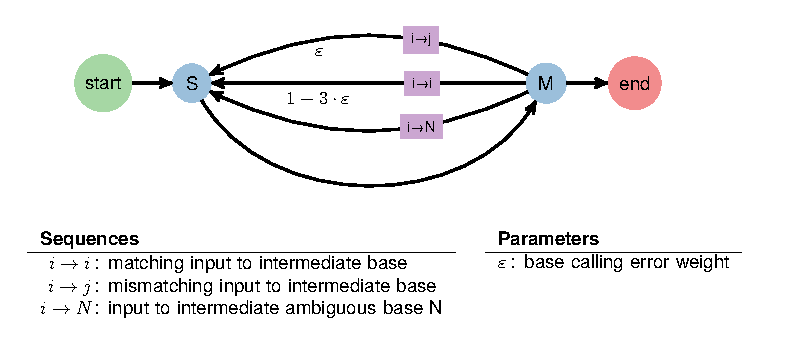
\includegraphics{figures/fig-base-calling-error.pdf}
\caption{\label{fig:figs} Base calling error FST. Arcs from M to S
generate matches; however, here they can introduce single-nucleotide
errors, which can generate stop codon artifacts.}
\end{figure}

\begin{figure}

{\centering 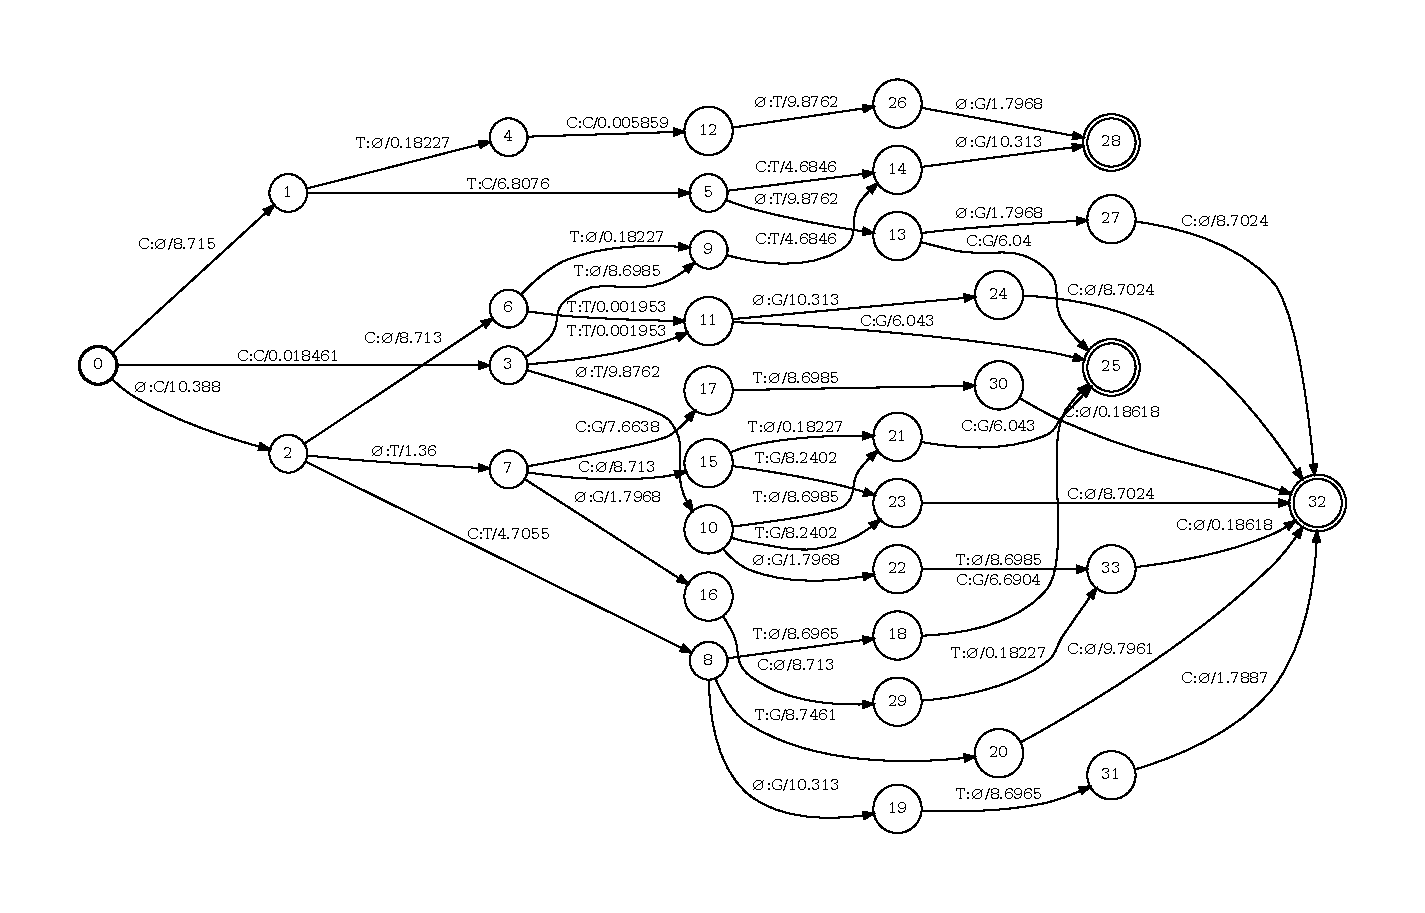
\includegraphics{figures/aln-example-graph} 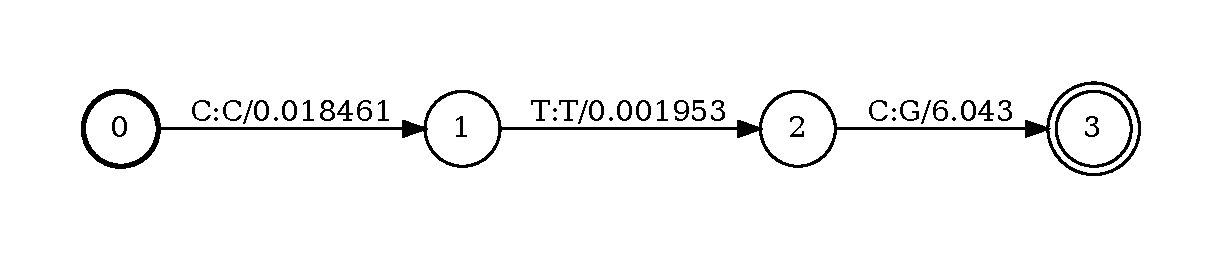
\includegraphics{figures/aln-example} 

}

\caption{\label{fig:aln-example} FST of all possible alignments between `CTC' and `CTG' (top) and the best alignment, determined by the shortest path (bottom). Figures generated using the OpenFST library.}\label{fig:aln-example}
\end{figure}

\begin{figure}

{\centering 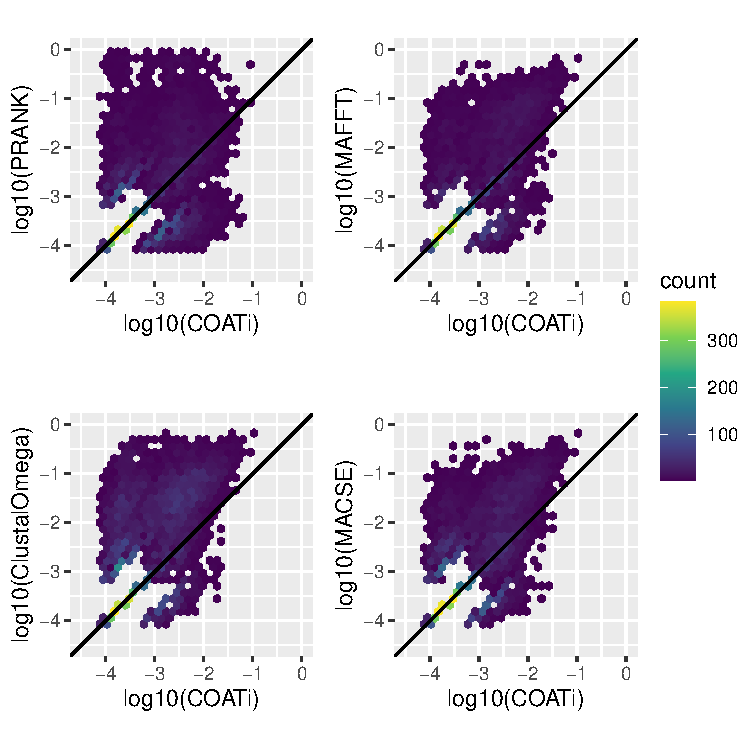
\includegraphics{figures/dseq_plots_tri-mg} 

}

\caption{\label{fig:dseq-tri-mg} Comparison of log10-transformed $d_{seq}$ data with pseudocounts between COATi codon-triplet-mg and PRANK, MAFFT, ClustalOmega, and MACSE. COATi was significantly more accurate than other aligners; all p-values were $\leq 1.25e-76$.}\label{fig:dseq1}
\end{figure}

\begin{figure}

{\centering 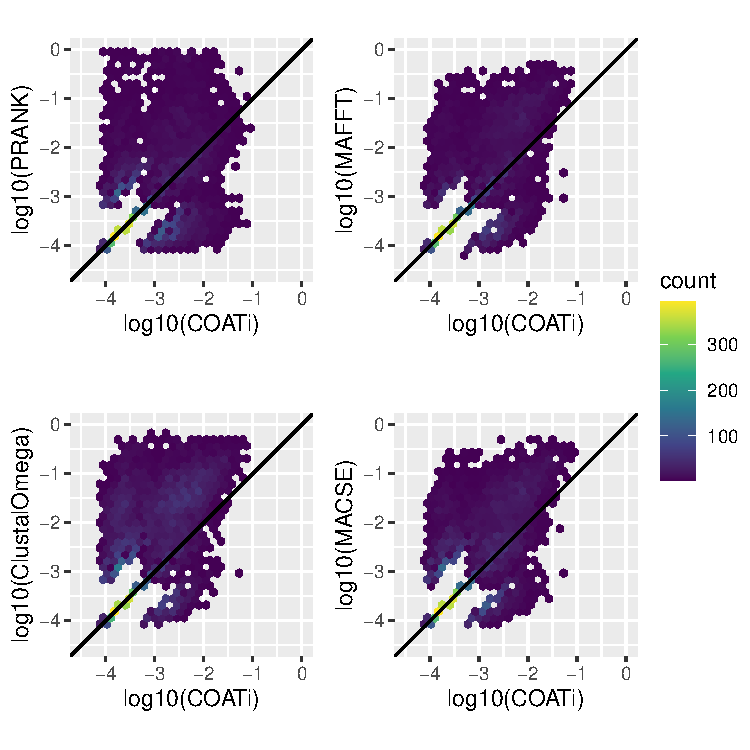
\includegraphics{figures/dseq_plots_tri-ecm} 

}

\caption{\label{fig:dseq-tri-ecm} Comparison of log10-transformed $d_{seq}$ data with pseudocounts between COATi codon-triplet-ecm and PRANK, MAFFT, ClustalOmega, and MACSE. COATi was significantly more accurate than other aligners; all p-values were $\leq 3.23e-48$.}\label{fig:dseq2}
\end{figure}

\begin{figure}

{\centering 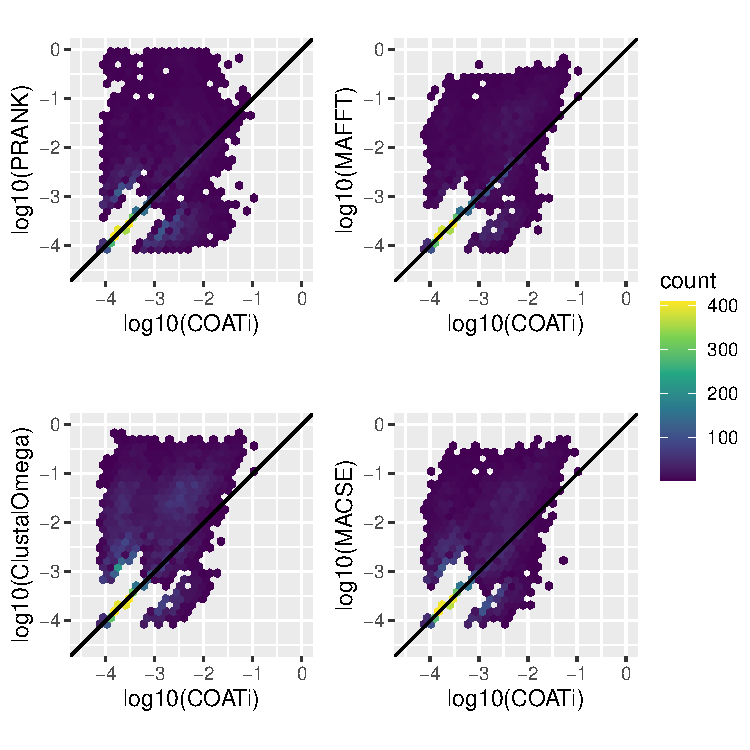
\includegraphics{figures/dseq_plots_mar-mg} 

}

\caption{\label{fig:dseq-mar-mg} Comparison of log10-transformed $d_{seq}$ data with pseudocounts between COATi codon-marginal-mg and PRANK, MAFFT, ClustalOmega, and MACSE. COATi was significantly more accurate than other aligners; all p-values were $\leq 1.99e-53$.}\label{fig:dseq3}
\end{figure}

\begin{figure}

{\centering 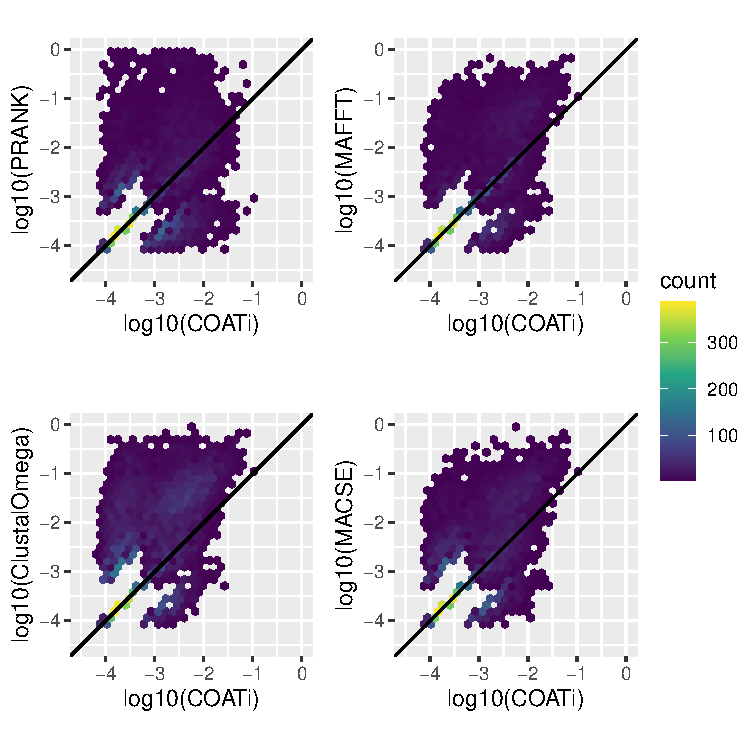
\includegraphics{figures/dseq_plots_mar-ecm} 

}

\caption{\label{fig:dseq-mar-ecm} Comparison of log10-transformed $d_{seq}$ data with pseudocounts between COATi codon-marginal-ecm and PRANK, MAFFT, ClustalOmega, and MACSE. COATi was significantly more accurate than other aligners; all p-values were $\leq 1.44e-52$.}\label{fig:dseq4}
\end{figure}

\begin{figure}

{\centering 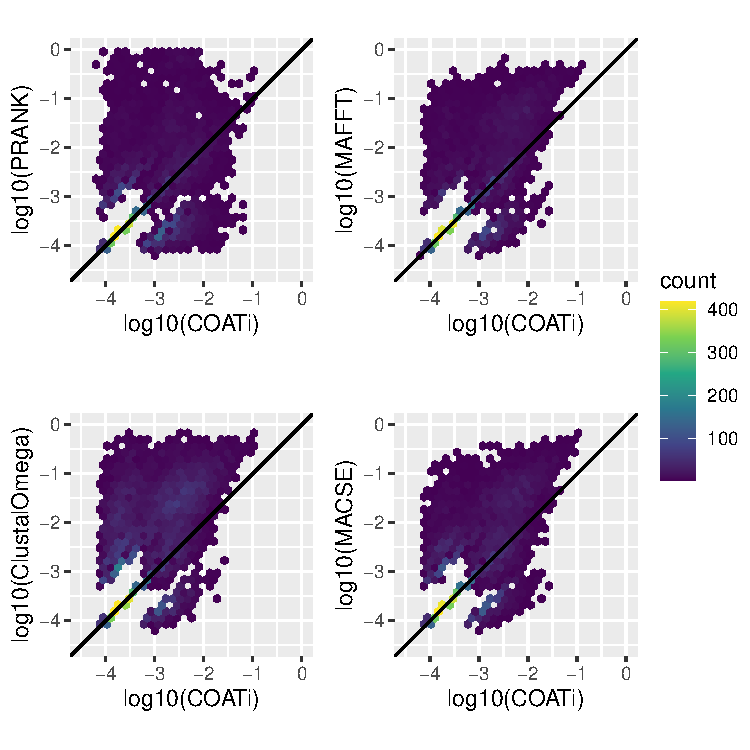
\includegraphics{figures/dseq_plots_reverse} 

}

\caption{\label{fig:dseq-reverse} Comparison of log10-transformed $d_{seq}$ data with pseudocounts between COATi codon-triplet-mg and PRANK, MAFFT, ClustalOmega, and MACSE with gorilla as the reference. COATi was significantly more accurate than other aligners; all p-values were $\leq 1.75e-64$.}\label{fig:dseq5}
\end{figure}

\newpage

\begin{figure}
\centering
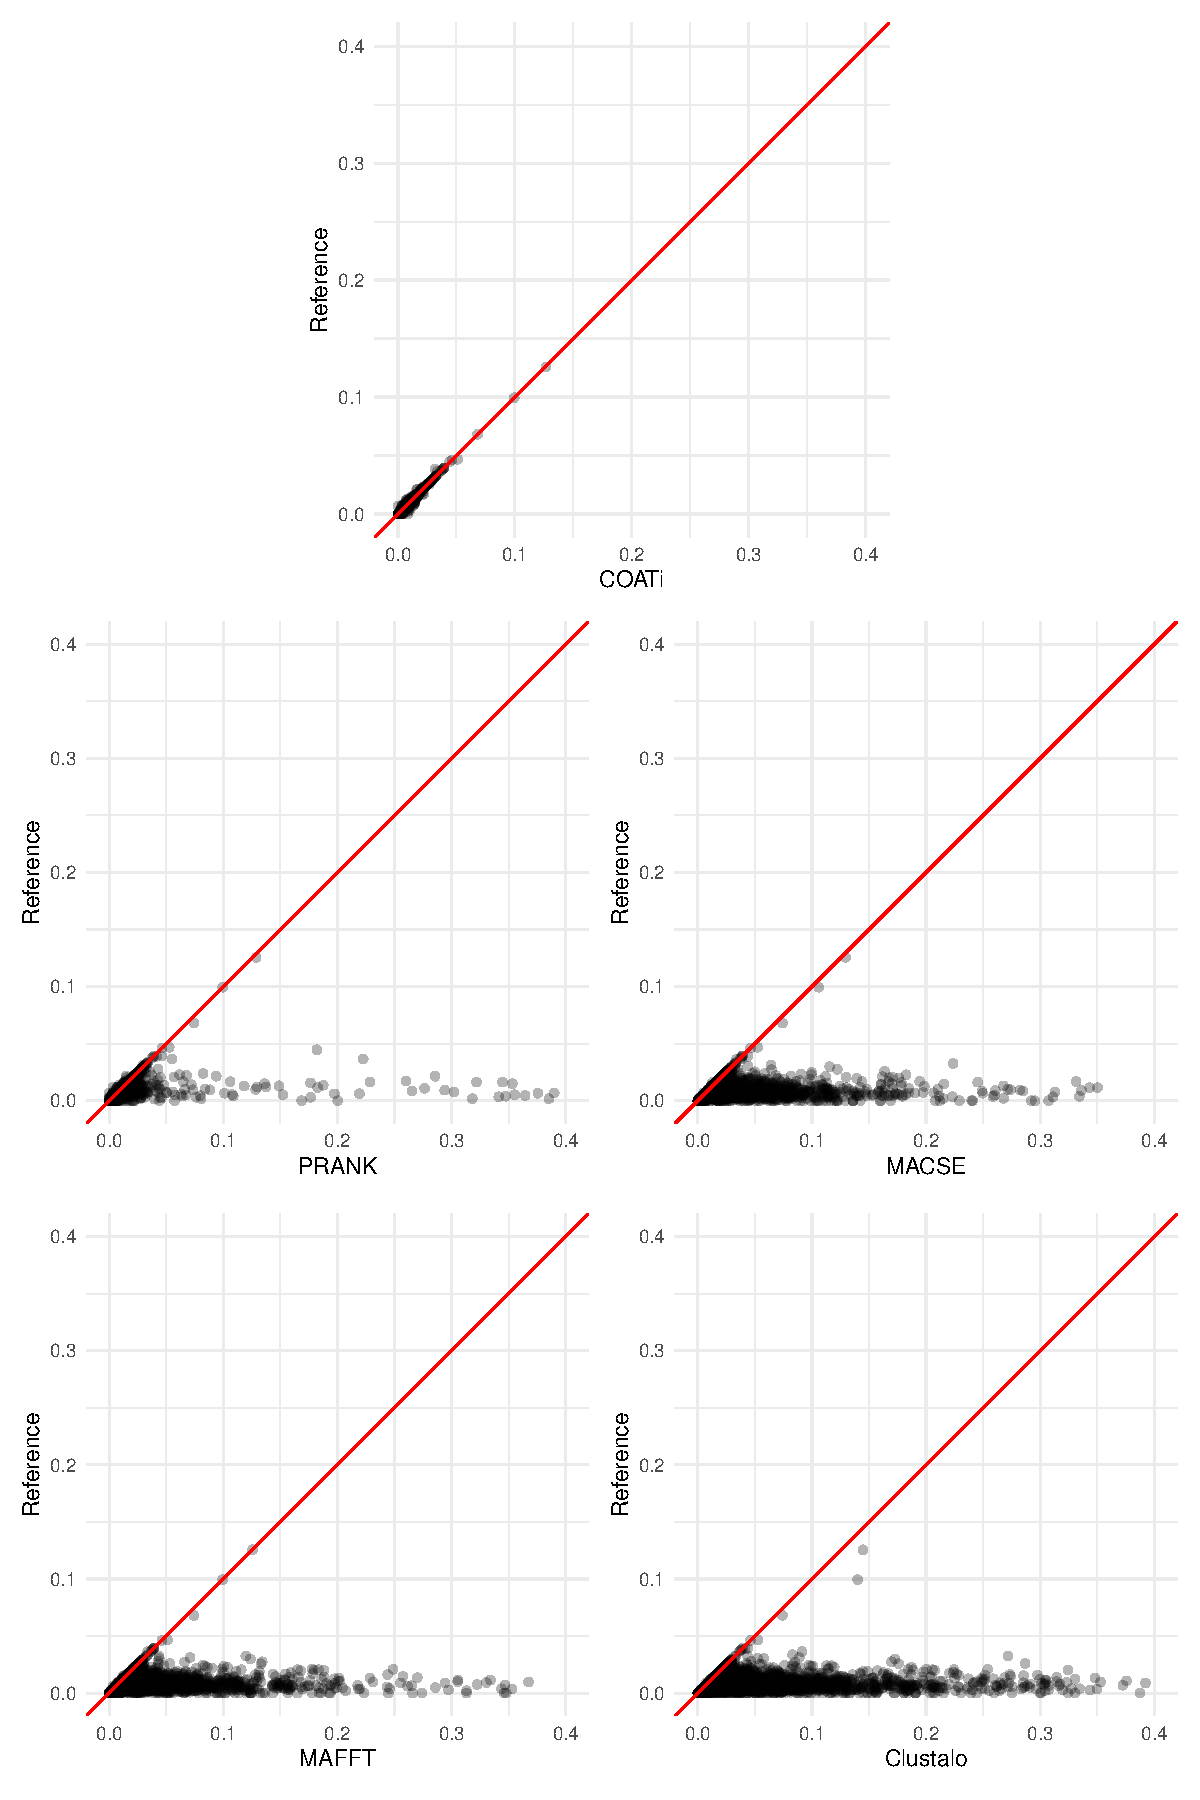
\includegraphics{figures/k2p_distances.pdf}
\caption{\label{fig:k2p} K2P distances. Evolutionary distances between
reference and retrieved alignments for each method calculated using the
Kimura 2-parameter model. Notably, COATi performs best while the other
tools tend to overestimate the evolutionary distance.}
\end{figure}

\end{document}
